%%%%%%%%%%%%%%%%%%%%%%%%%%%%%%%%%%%%%%%%%%%%%%%%%%%%%%%%%%%

\chapter{Modello del sistema}
\label{ref:modSistema}

%%% Il gruppo 1 scriverà il suo modello del sistema. Esso dovrà includere: attori, casi d'uso (descrizione e tabella), scenari, diagrammi dei casi d'uso, diagrammi di sequenza, diagramma delle attività, screen mockups della funzionalità %%%

\section{Attori}
\label{sec:attori}
\subsection{\textit{Sync}}
\paragraph{} 
\textit{Sync} rappresenta il sincronizzatore remoto, un web service esterno che si interfaccia con una serie di servizi tra cui \textit{Esse3}, ossia il portale dello studente che offre le funzionalità da replicare nell’applicazione, \textit{Aule Unimol} ed altri servizi esterni. È un’entità esterna al sistema che si vuole realizzare, pertanto  è classificata come attore.
\begin{center}
	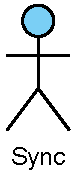
\includegraphics[width=0.6in]{imgs/attori/Attore-Sync.pdf}
\end{center}

\subsection{\textit{Docente}}
\paragraph{} 
\textit{Docente} è un professore dell’\textit{Università degli Studi del Molise} avente le credenziali di accesso al portale \textit{Esse3}. Il \textit{Docente} utilizzerà la nuova funzionalità per comunicare in modo rapido e semplice e anche in via ufficiosa con tutti gli studenti che frequentano un proprio corso. Egli potrà amministrare le chat secondo le sue preferenze, in particolare potrà creare o rimuovere dei canali e aggiungere o rimuovere i membri.
\begin{center}
	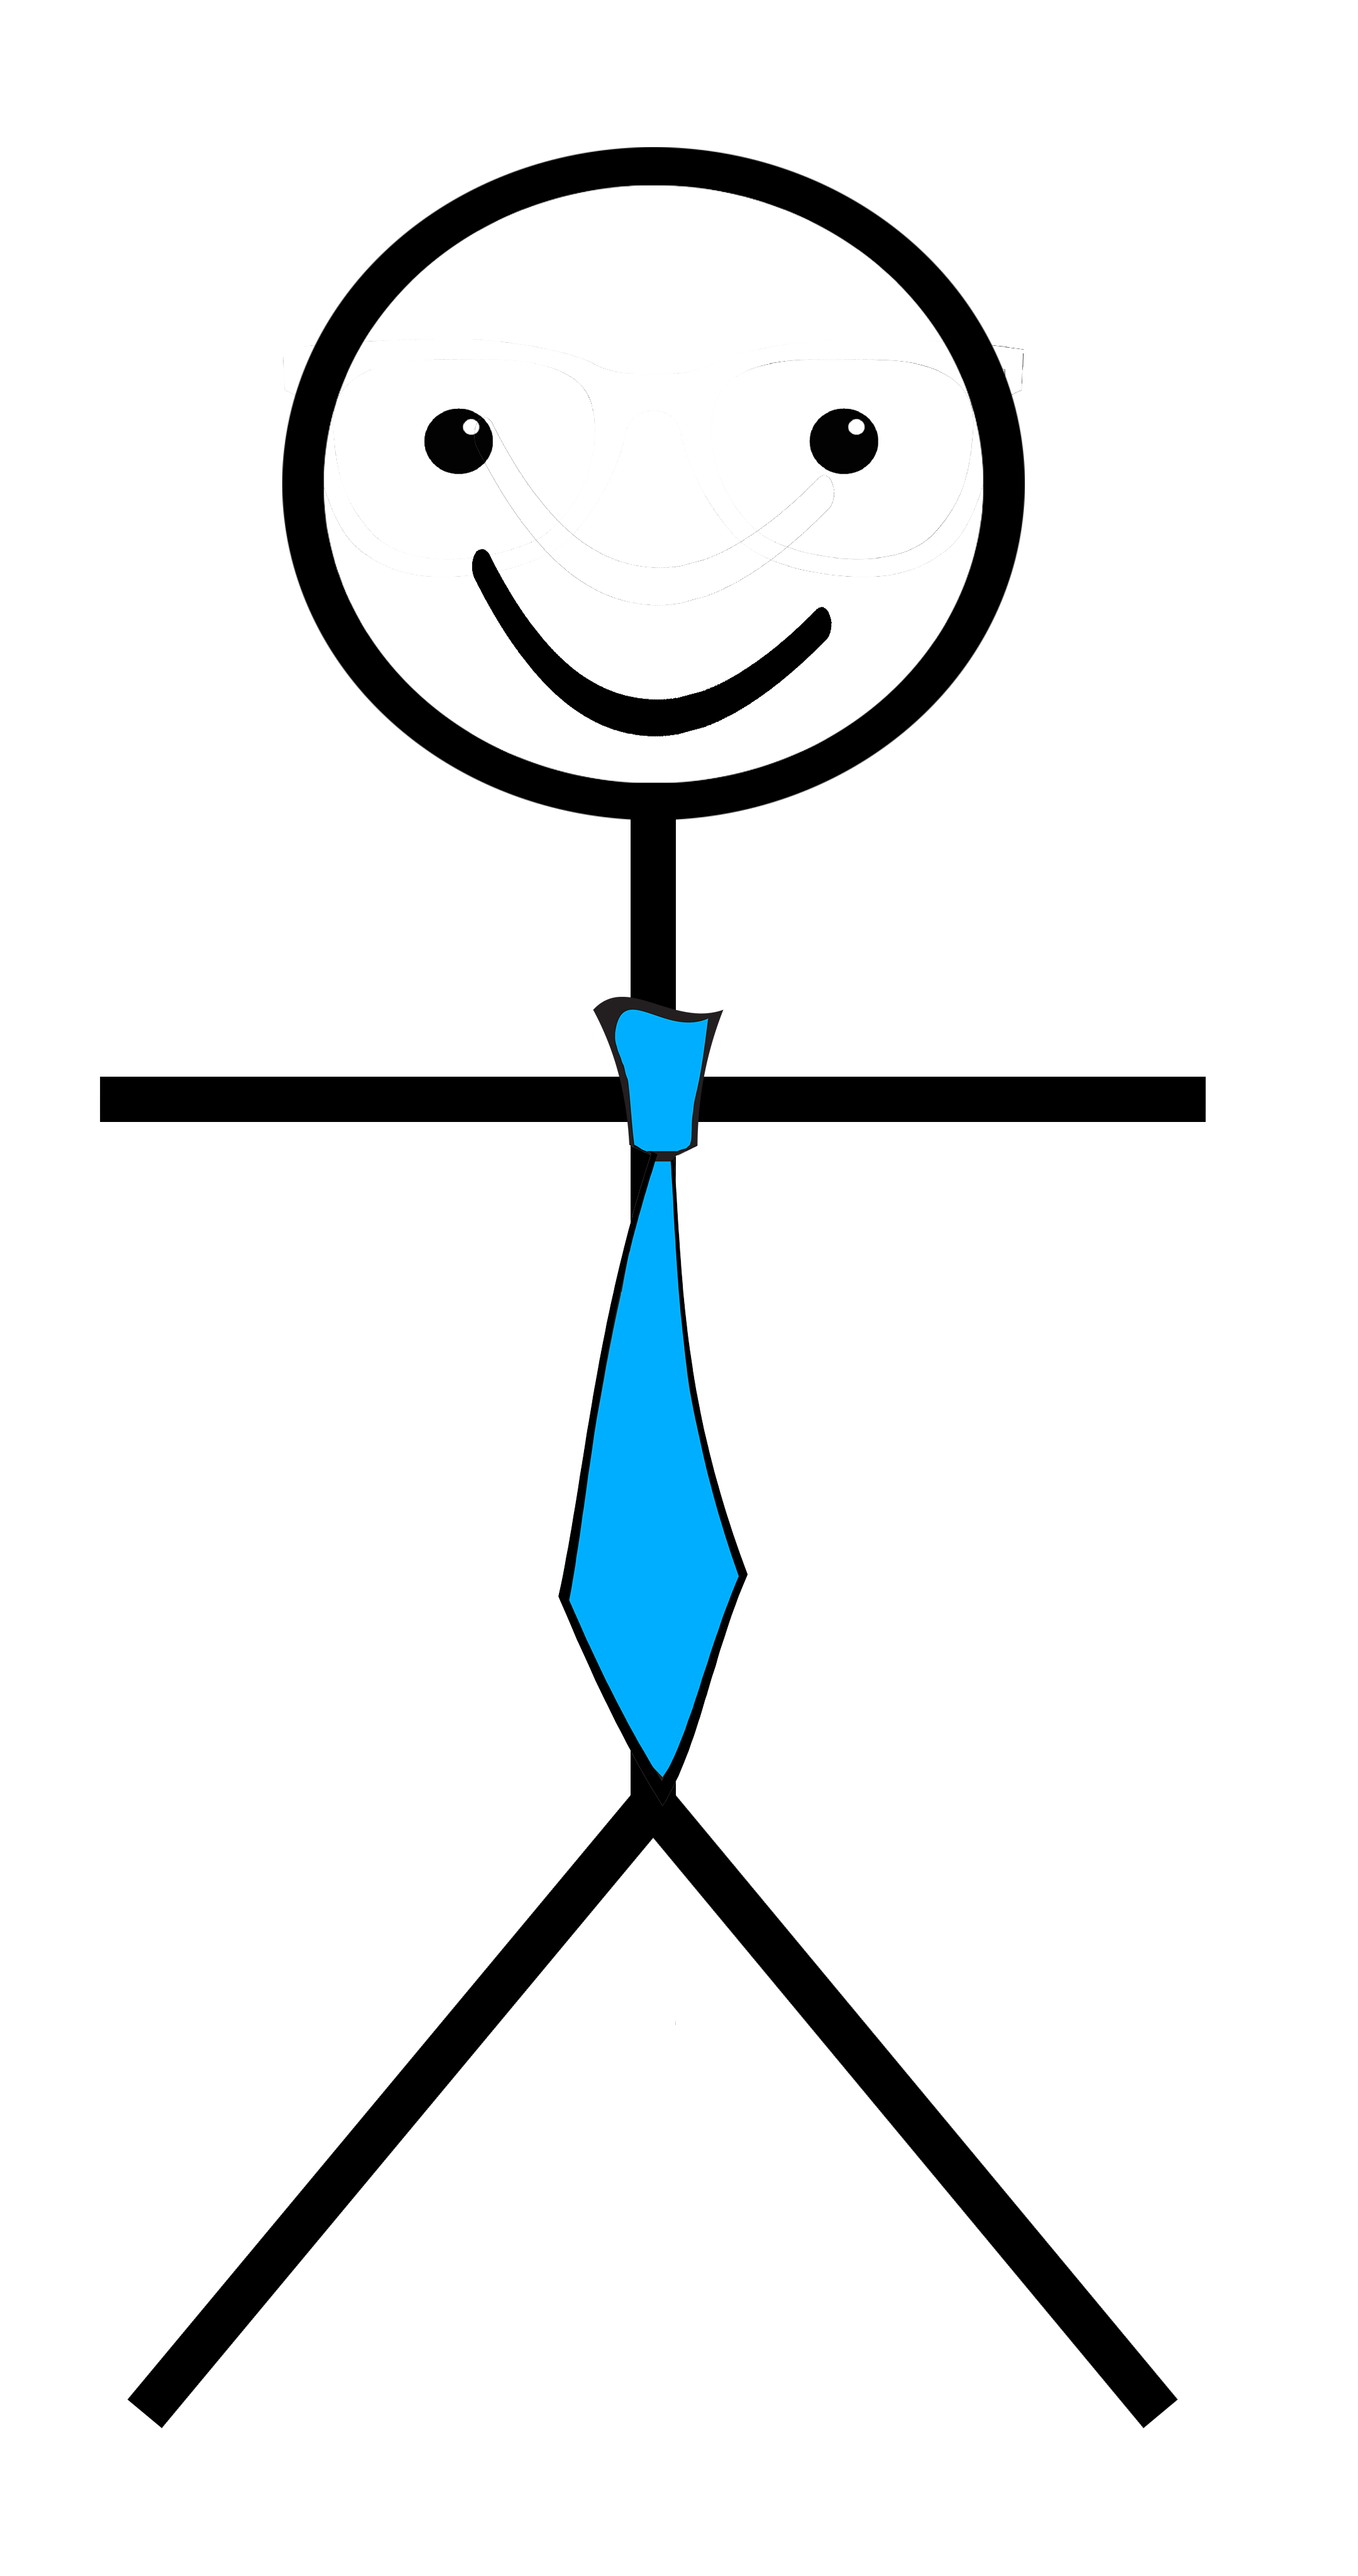
\includegraphics[width=0.6in]{imgs/attori/Docente.png}
\end{center}

\subsection{Studente}
\paragraph{} 
Studente regolarmente iscritto all’\textit{Università degli Studi Del Molise}, munito delle credenziali per accedere al portale dello studente \textit{Esse3}, il servizio esterno sul quale si basa l’applicazione. Lo studente utilizza l’applicazione per usufruire in maniera agevole dei servizi offerti dai portali dell’\textit{Università degli Studi del Molise} e monitorare la propria carriera universitaria. Di seguito è mostrata l'icona dello studente standard.
\begin{center}
	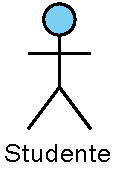
\includegraphics[width=0.8in]{imgs/attori/Attore-Studente.pdf}
\end{center}
Per quanto riguarda la nuova funzionalità di messaggistica, lo \textit{Studente} utilizzerà tale funzione per facilitare la comunicazione ufficiale con i docenti relativi ai corsi della Coorte di appartenenza. Potrà comunicare, inoltre, con gli altri studenti appartenenti al suo stesso anno di corso. Di seguito è mostrato lo studente della chat.
\begin{center}
	
\includegraphics[width=0.8in]{imgs/attori/Studente.png}
	\label{fig:Attore: Studente chat}
\end{center}


\emph{\textbf{Amministratore:} è un Amministratore dell’Università degli Studi del Molise}, al quale sono assegnate le credenziali per poter effettuare l’accesso al pannello amministrazione.\emph{L’Amministratore} avrà il compito di gestire, mediante tale pannello, le \emph{chat} degli studenti e le \emph{chat} dei corsi dove potrà coordinare i relativi canali e gli utenti in essi presenti.
Avrà anche la possibilità di inviare notifiche personalizzate e di gestire la segnalazione dei messaggi inopportuni all’interno delle \emph{chat}.

\begin{figure}[h]
	\centering
	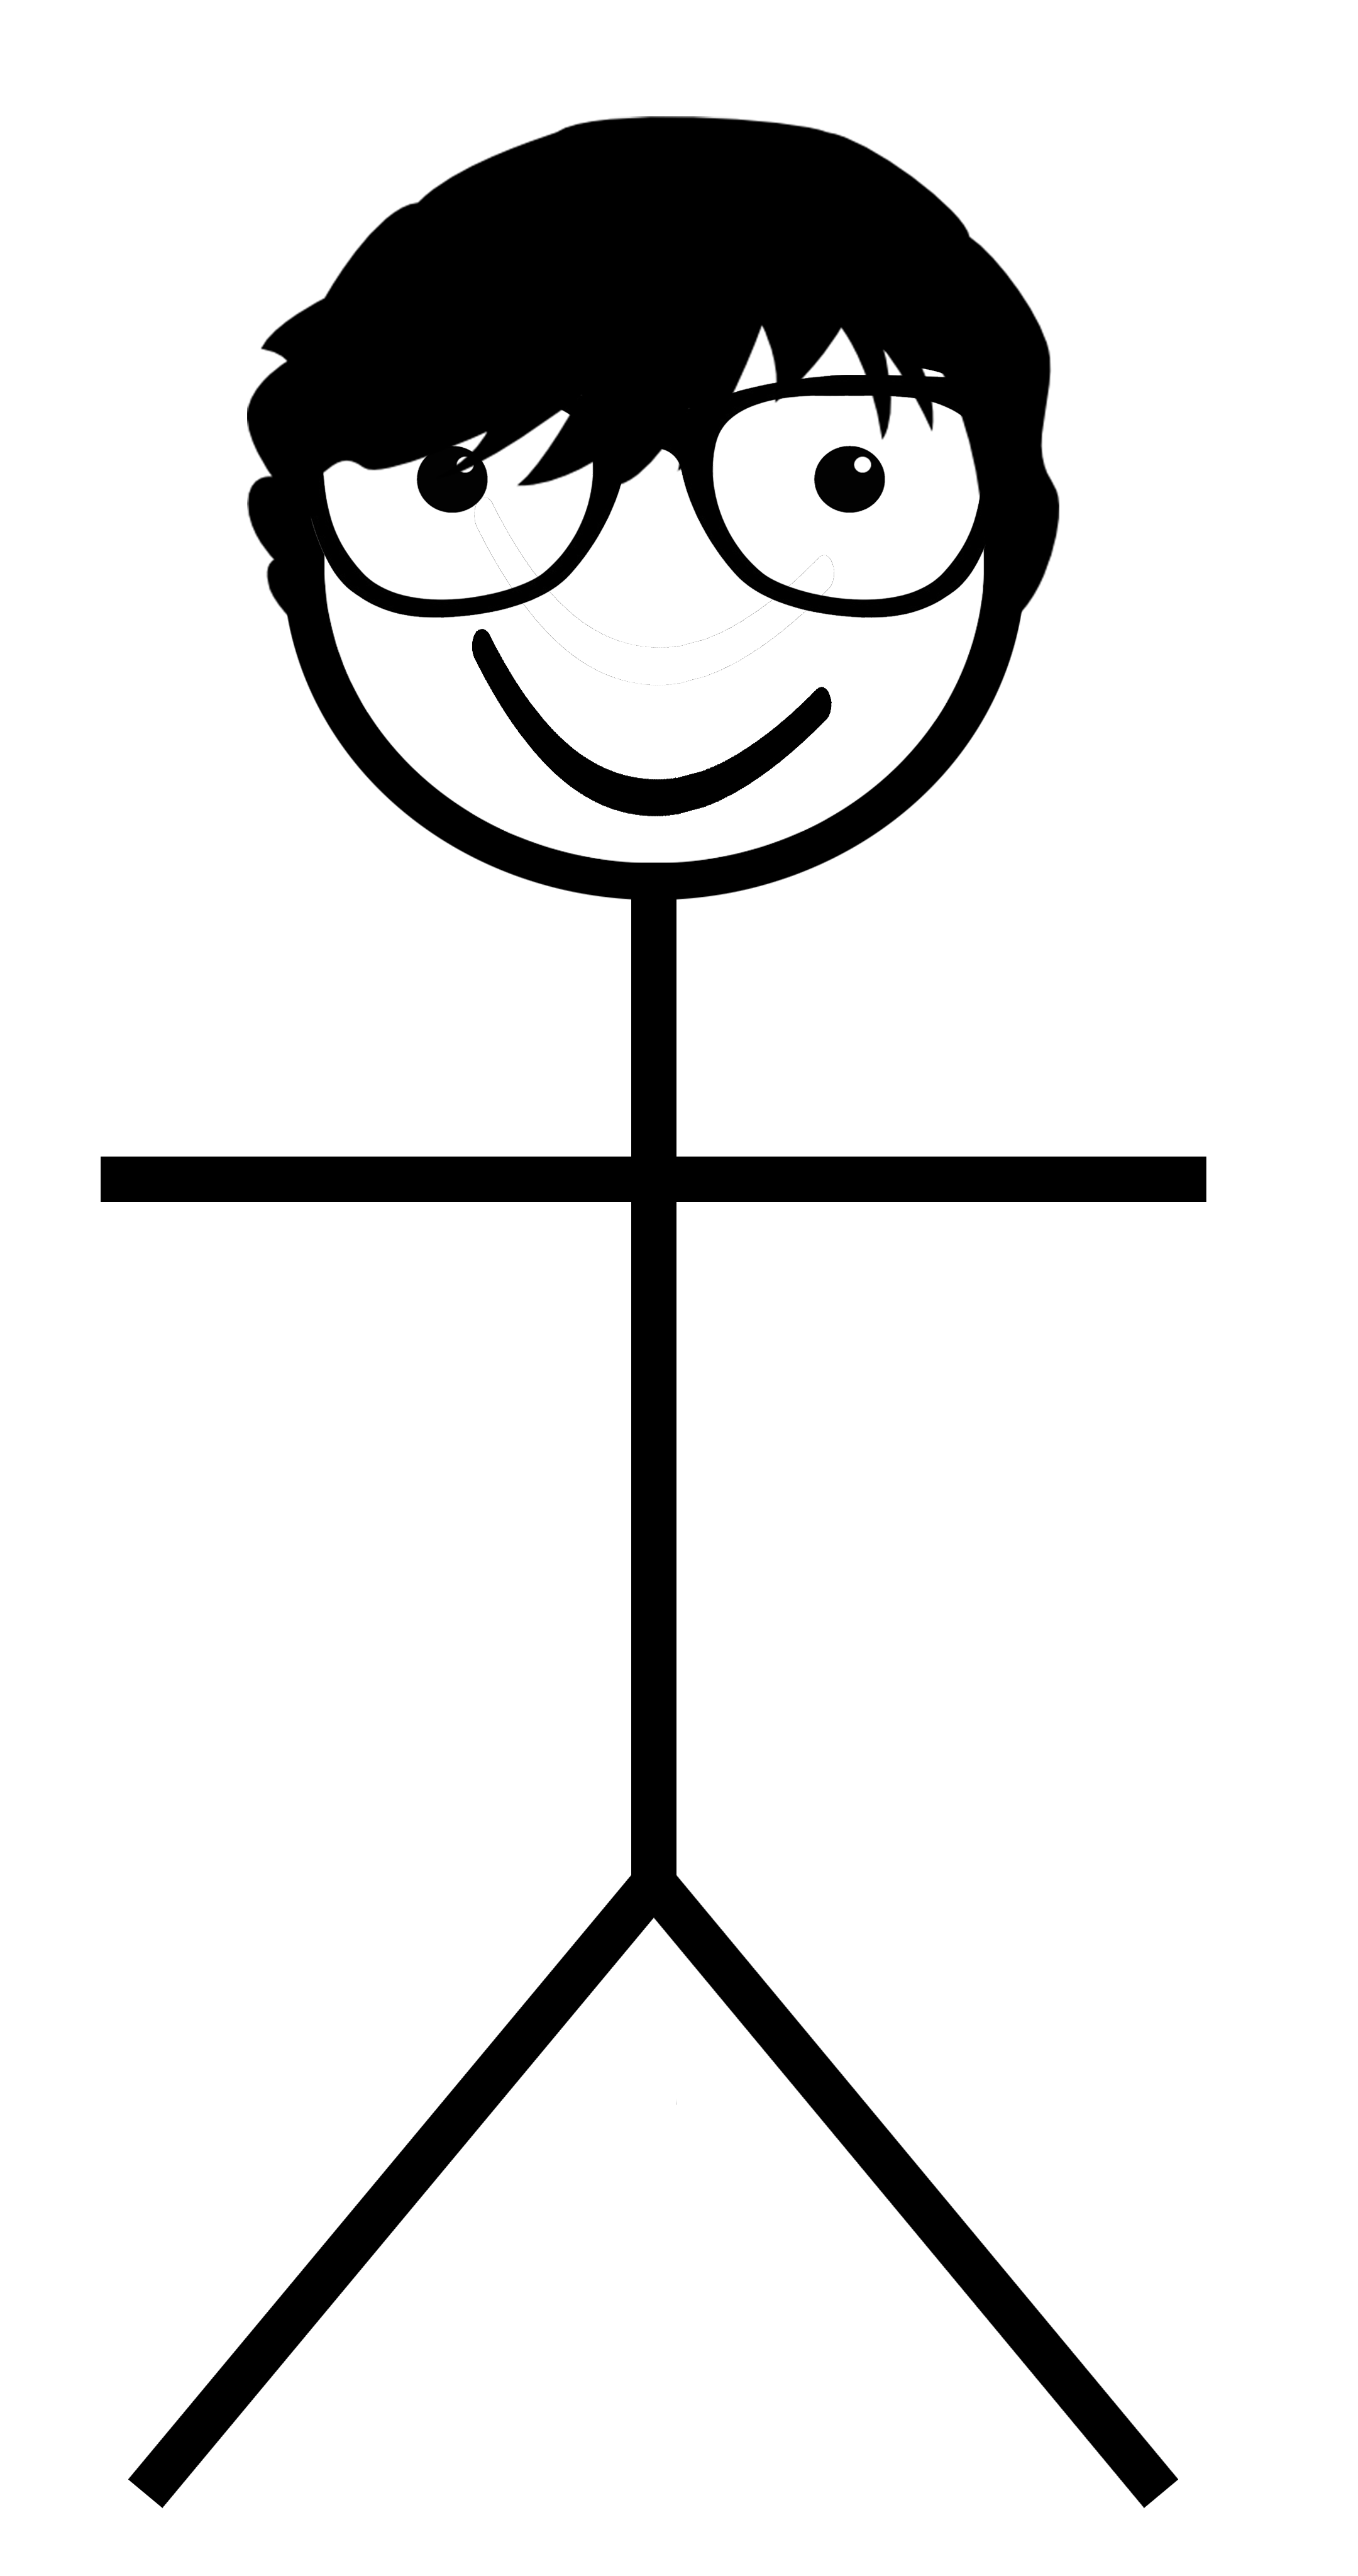
\includegraphics[width=0.2\textwidth]{imgs/attori/admin.png}
	\caption{Attore: Amministratore}
	\label{fig:Attore: Amministratore} 
\end{figure}



\newpage


\section{Scenari}
Inserire qui gli scenari di tutti i gruppi.

\section{Casi d'uso}
Inserire casi d'uso di tutti i gruppi.

\paragraph{Caso d'uso 1 (sostituire con nome caso d'uso) \\} 
Lorem ipsum dolor sit amet... (sostituire con descrizione caso d'uso)

\begin{table}[tb]
%\normalsize % Dimensione testo normale
\small % Dimensione testo piccola
%\footnotesize % Dimensione testo piccolissima
%\scriptsize % Dimensione del testo ulteriormente più piccola
%\caption{} % Didascalia tabella
%\label{} % Etichetta per riferimenti incrociati
\begin{tabular}{| p{\useCaseLeft} | p{\useCaseNum} | p{\useCaseTwoCol} | p{\useCaseTwoCol} |}
	\hline
	\textbf{Nome caso d'uso} & \multicolumn{3}{p{\useCaseMulticol} |}{\textbf{Login}} \\
	\hline
	\textbf{Attori partecipanti} & \multicolumn{3}{p{\useCaseMulticol} |}{Inizializzato da \textbf{Utente}.} \\
	\hline
	\textbf{Condizioni d'ingresso} & \multicolumn{3}{p{\useCaseMulticol} |}{L'utente ha cliccato sul bottone di login.} \\
	\hline
	\textbf{Flusso degli eventi} & \textbf{\#} & \textbf{Utente} & \textbf{Sistema} \\
	\hline
	\textbf{} & \textbf{1} & \textbf{} & Propone una schermata per l'inserimento dei dati necessari per il login, e-mail e password dell'utente \\
	\hline
	\textbf{} & \textbf{2} & Inserisce i dati e sottomette la richiesta & \textbf{} \\
	\hline
	\textbf{} & \textbf{3} & \textbf{} & Controlla che siano stati inseriti entrambi i campi e avvia le operazioni di visualizzazione \\
	\hline
	\textbf{Eccezioni} & \multicolumn{3}{p{\useCaseMulticol} |}{3.1 Uno o entrambi i campi sono vuoti.\newline 3.2 Le credenziali inserite non sono valide (una o entrambe).} \\
	\hline
	\textbf{Condizioni d'uscita} & \multicolumn{3}{p{\useCaseMulticol} |}{Il sistema completa la login e dà accesso all'app o, in caso contrario, visualizza un messaggio di errore se non sono stati inseriti tutti i dati obbligatori, se le credenziali non sono corrette o se si verifica un insuccesso dell'operazione.} \\
	\hline
\end{tabular}
\end{table}

\section{Diagramma dei casi d'uso}

Inserire diagramma casi d'uso di tutti i gruppi.

\begin{figure}
	\centering
	%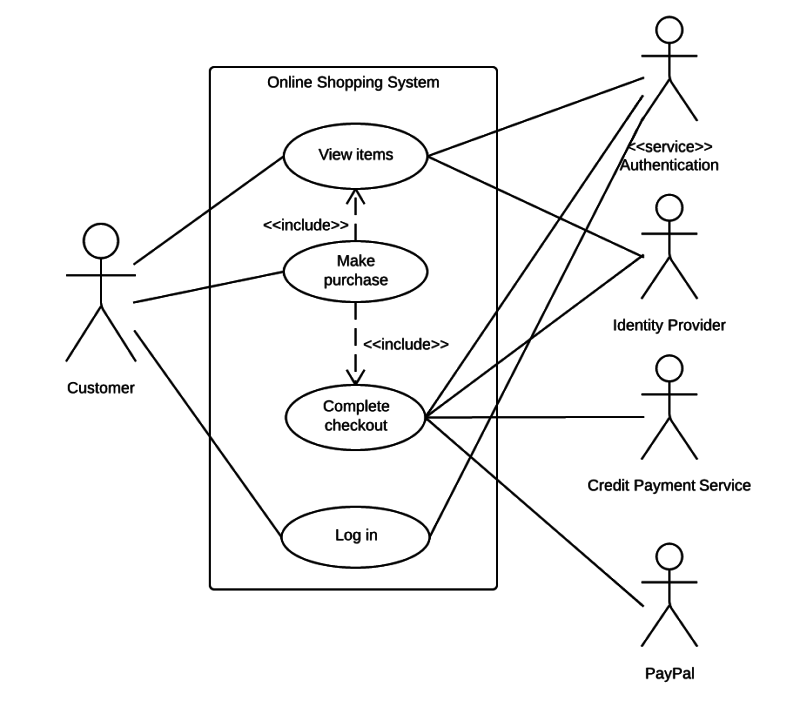
\includegraphics[height=3in]{imgs/file-comuni-ai-gruppi/useCaseEsempio.png}
	\caption{Inserire descrizione}
	\label{fig:prova}
\end{figure}

\section{Diagramma di sequenza}

Inserire diagrammi di sequenza di tutti i gruppi.

\begin{figure}
	\centering
%	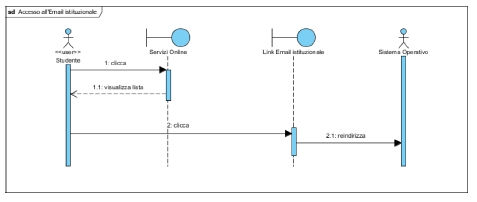
\includegraphics[height=3in,width=5in]{imgs/file-comuni-ai-gruppi/SequenceDgEsempio.png}
	\caption{Inserire descrizione}
	\label{fig:prova}
\end{figure}

\section{Diagramma delle attività}

Inserire diagrammi di activity di tutti i gruppi.

\begin{figure}
	\centering
%	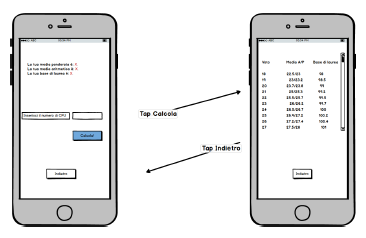
\includegraphics[height=3in,width=5in]{imgs/file-comuni-ai-gruppi/ActivityDgEsempio.png}
	\caption{Inserire descrizione}
	\label{fig:prova}
\end{figure}



\clearpage